\documentclass{article}
\usepackage[utf8]{inputenc}

\title{TT3010 - Audio technology and room acoustics. \newline Exercise 3 - Loudspeakers \newline Solutions}

\author{Jan Arne Bosnes}
\date{\today}

\usepackage{natbib}
\usepackage{graphicx}
\usepackage{float}

\begin{document}

\maketitle

\section*{Tasks}

\subsection*{1}

The difference in power output level, in dB is,

\begin{equation}
    \Delta L_W = L_2 - L_1 = 10\log(\frac{P_2}{P_1})
\end{equation}
where $P_1$ and $P_2$ are the sound powers of the two loudspeakers.

\noindent The acoustic power output, $P$, for a received electrical power $P_e$, with an efficiency of $\eta$, is

\begin{equation}
    P= \eta P_e
\end{equation}

Since both speakers receive the same electrical power input, the expressions for the sound power are

\begin{equation}
    P_1= \eta_1 P_e
\end{equation}

\begin{equation}
    P_2= \eta_2 P_e
\end{equation}
where $\eta_1$ and $\eta_2$ are respective efficiency of loudspeakers.

We can then combine the equations to get the following,

\begin{equation}
    \Delta L_W = 10\log(\frac{\eta_2 P_e}{\eta_1 P_e}) = 10\log(\frac{10 \%}{ 1 \%}) = 10 \log(10) = 10 \ {\rm dB}
\end{equation}

Therefore, the loudspeaker with 10 \% efficiency will radiate a 10 dB higher level than the loudspeaker with 1 \% efficiency.

\subsection*{2}

The cone of a speaker can be taken as circular in shape. The area of a circle is related to its radius as $A=\pi r^2$, where $A$ is the area, and $r$ is the radius of the cone. The radius is half of the diameter ($d$), which then gives us the following,
\begin{equation}
    A=\pi (\frac{d}{2})^2 = \frac{\pi d^2}{4}
    \label{eq:areal}
\end{equation}

The areas are as follow
\begin{equation}
    A_{20 cm} = 100 \pi {\rm cm}^2, \ A_{30 cm} = 225 \pi {\rm cm}^2, \ A_{38 cm} = 361 {\rm cm}^2
\end{equation}

So, the ratio between those speaker cones would be 
\begin{equation}
    A_1 : A_2 : A:3 = 100:225:361
\end{equation}



\subsection*{3}

The sound waves will have to travel from the center of the frontal side to the center of the back of the baffle, as shown in figure \ref{fig:baffel} since the loudspeaker is mounted at the centre of the baffle.

\begin{figure}[H]
    \centering
    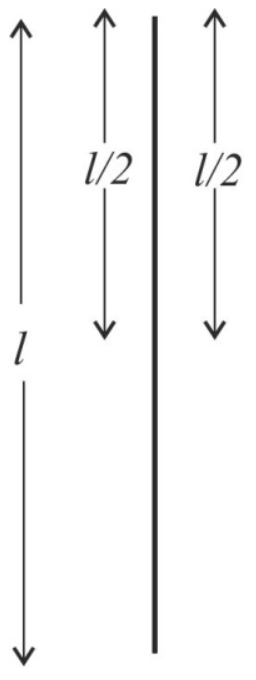
\includegraphics{figures/oving3_1_solutions.png}
    \caption{Baffle of sidelength $l$.}
    \label{fig:baffel}
\end{figure}

\subsubsection*{a}

The sound wave must travel twice the half-length of the board. Therefore, the path length $x$ from the center of the frontal side to the center of the back of the baffle is,

\begin{equation}
    x = 2 \frac{l}{2}+l = 2l
\end{equation}

The length of the baffle is 1 m. Hence, the length $x = 1 $ m.

\subsubsection*{b}

The wavelength $\lambda$, frequency $f$, and speed of sound $c$ are related as,

\begin{equation}
    \lambda = \frac{c}{f}
\end{equation}

In a, we saw that the sound wave must have the wavelength $\lambda = 2l$. We can then rewrite the frequency in terms of speed and length of baffle.

\begin{equation}
    f=\frac{c}{2l}
\end{equation}

This will give us a frequency $f=170$  Hz.

\subsection*{4}

\subsubsection*{a}
\begin{figure}[H]
    \centering
    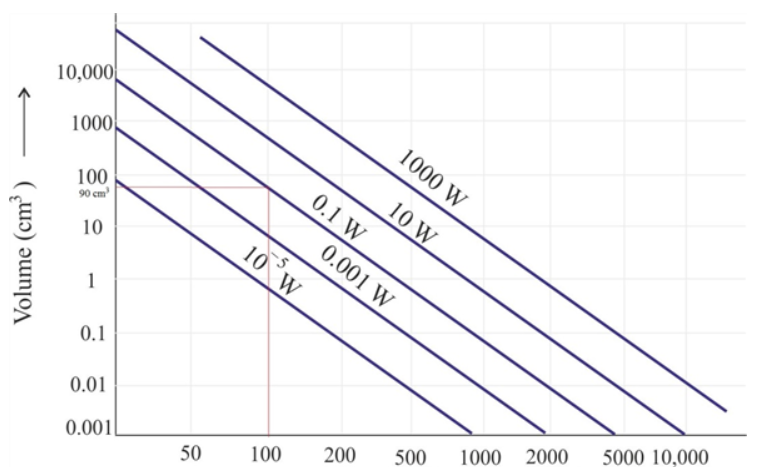
\includegraphics[scale = 1.4]{figures/oving3_2_solutions.png}
    \caption{Approximately measurement of the volume at given frequency drives a certain power.}
    \label{fig:loudsp}
\end{figure}

As shown in figure \ref{fig:loudsp}, we can approximately say that 90 cm$^3$ must be moved in order to radiate 0.1 W power at 100 Hz.

\subsubsection*{b}

The air in front of the speaker cone can be considered as a cylinder. Thus, the volume of the air moved must be equal to the product of the area of the cone and the cone excursion. If the cone with an area $A$ moves a distance $l$, then the volume of air moved is,

$V=Al$
where the area of the cone is related to its radius $r$ as (see task 2),

\begin{equation}
    A=\pi r^2
\end{equation}

which will give us
\begin{equation}
    V=\pi r^2 l
\end{equation}

Since the radius is half the diameter, we can use formula (\ref{eq:areal}) from task 2:

\begin{equation}
    V=\frac{\pi d^2}{4}l
\end{equation}

By rearranging the equation, we get:

\begin{equation}
    l=\frac{4V}{\pi d^2}
    \label{eq:distance_speaker}
\end{equation}

If we insert the numerical values for $V$ and $d$, this gives us $l \approx 0.28 \ cm$, which is the distance the cone must move to radiate 0.1 W of acoustic power at 100 Hz. 

\subsection*{5}

It is given in the task that $L_w = L_p+8$, so $L_w = 100 $ dB. By reformulating the formula for the sound power level and knowing that the reference power, $W_0 =10^{-12}$ W, we get the following,
\begin{equation}
    L_W=10 \log{\frac{W}{W_0}} \rightarrow W=W_0 \cdot 10^{\frac{100}{10}} = 10^{-2} W
\end{equation}

We can then calculate the efficiency $\eta  = \frac{W}{W_{produced}} = \frac{10^{-2}}{1} = 1 \%$


\subsection*{6}

\begin{figure}[H]
    \centering
    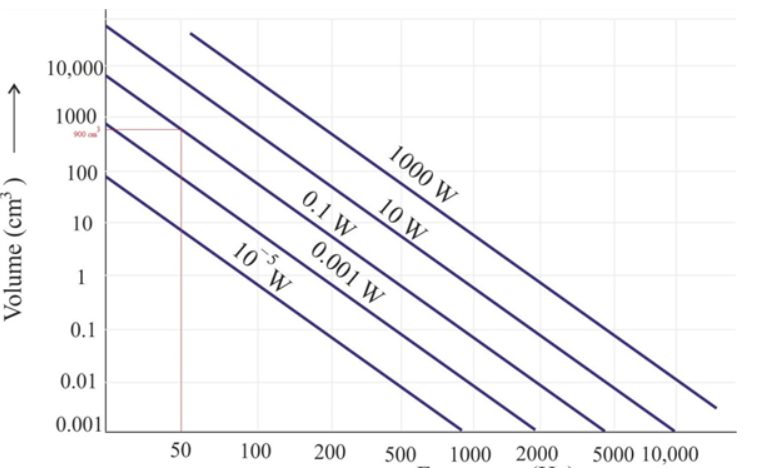
\includegraphics[scale=1.5]{figures/oving3_3_solutions.png}
    \caption{Approximately measurement of the volume at given frequency drives a certain power.}
    \label{fig:loudspeaker}
\end{figure}

Figure \ref{fig:loudspeaker} shows us that approximately 900 cm$^3$ of air must be moved in order to radiate 0.1 W power at 50 Hz.

This is the same procedure as we did in task 4. We use equation (\ref{eq:distance_speaker}) to retrieve the distance that the cone must move in order to radiate 0.1 W of acoustic power at 50 Hz.

\begin{equation}
    l=\frac{4V}{\pi d^2}=\frac{4 \cdot 900 cm^3}{\pi (30.48 cm)^2} = 1.2 cm
\end{equation}

\subsection*{7}

The resonance frequency of a loudspeaker is given in terms of its compliance  and mass of driver as,

\begin{equation}
    f_d =\frac{1}{2 \pi \sqrt{C m} }
\end{equation}
where $f_d$ is the resonance frequency, $C$ is the compliance of the loudspeaker driver, and $m$ is the mass. 
The mass of the cone and voice coil is 71 g = 7.1 $\cdot 10^{-2}$ kg. So, this gives us the following resonance frequency:

\begin{equation}
    f_d \approx 20 Hz
\end{equation}

%\bibliographystyle{plain}
%\bibliography{references}
\end{document}
